\documentclass[10pt, conference, letterpaper, compsocconf]{IEEEtran}
\usepackage[T1]{fontenc}
\usepackage[latin9]{inputenc}
\usepackage{amsmath}
\usepackage{amssymb}
\usepackage{subscript}
\usepackage{color}


\makeatletter

%%%%%%%%%%%%%%%%%%%%%%%%%%%%%% LyX specific LaTeX commands.
%% Because html converters don't know tabularnewline
\providecommand{\tabularnewline}{\\}

\newcommand{\todoc}[2]{{\textcolor{#1} {\textbf{[[#2]]}}}}
\newcommand{\todo}[1]{{\todoc{red}{\textbf{[[#1]]}}}}

\newcommand{\todored}[1]{\todoc{red}  {\textbf{[[#1]]}}}
\newcommand{\todoblue}[1]{\todoc{blue}{\textbf{[[#1]]}}}
\newcommand{\todogreen}[1]{\todoc{green}{\textbf{[[#1]]}}}
\newcommand{\todoorange}[1]{\todoc{DarkOrange}{\textbf{[[#1]]}}}
%% Additional todo commands:
\newcommand{\TODO}[1]{\todored{#1}}
\newcommand{\sung}[1]{\todored{Sung: #1}}
\newcommand{\shiv}[1]{\todoblue{Shiv: #1}}
\newcommand{\jim}[1]{\todoblue{Jim: #1}}

\newcommand{\zhongpeng}[2]{\todoblue{ZhongPeng: #2}}
%\newcommand{\pparagraph}{\paragraph {\indent}}

%%%%%%%%%%%%%%%%%%%%%%%%%%%%%% User specified LaTeX commands.
\@ifundefined{definecolor}
 {\usepackage{color}}{}
\definecolor{note_fontcolor}{rgb}{0.80078125, 0.80078125, 0.80078125}% \documentclass[10pt, conference, compsocconf]{IEEEtran}
% \documentclass[journal,10pt,draftclsnofoot,onecolumn]{IEEEtran}

% \documentclass{acm_proc_article-sp}
\usepackage{multirow}
\@ifundefined{definecolor}{\usepackage{color}}{}
\usepackage{algorithm}
\usepackage{threeparttable}
\usepackage{epsfig}
\usepackage{amsfonts}
\usepackage{cite}
\usepackage{array}


%\usepackage{babel}

\makeatother

\begin{document}

\title{Effective Bug Fix Suggestions}

\author{\IEEEauthorblockN{Shivkumar Shivaji \IEEEauthorrefmark{1},
Zhongpeng Lin \IEEEauthorrefmark{1}, E. James Whitehead, Jr. \IEEEauthorrefmark{1},
Ram Akella \IEEEauthorrefmark{1}, 
Sunghun Kim \IEEEauthorrefmark{2}}
\IEEEauthorblockA{ \IEEEauthorrefmark{1}School of Engineering\\
University of California Santa Cruz, \\
Santa Cruz, CA, USA\\
Email: \{shiv, ejw, ram\}@soe.ucsc.edu
}
\IEEEauthorblockA{ \IEEEauthorrefmark{2}Department of Computer Science\\
Hong Kong University of Science and Technology\\
Hong Kong\\
Email: hunkim@cse.ust.hk
}}

\maketitle
\jim{Author addresses -- go two column with these}

\begin{abstract}

Bug prediction techniques have evolved significantly in recent years.
While there has been considerable focus on detecting bugs, there is
less work on predicting the contents of a bug fix. We present a model
that predicts the contents of a future bug fix to a code change. Experiments
were conducted on four open source projects with large revision histories.

We start by analyzing the effectiveness of fix content prediction on future
code changes of a project. A classifier and a custom technique are then
used to generate potential fix content for bug inducing changes. Finally, human experts are consulted on hard to classify
bugs, and leveraged to improve predictions
on fix content.\end{abstract}
\begin{IEEEkeywords}
Empirical software engineering; Testing, verification, and validation;
Software analysis 
\end{IEEEkeywords}

\section{Introduction}
Many defect prediction techniques have been successfully explored in recent
years. These approaches are potentially accurate
enough for practical adoption. Some bug prediction methods can even
predict if a given software unit contains a defect. Examples of such techniques
can be found in \cite{Kim2007p58, shivaji2009reducing, aversano2007lbi, Hata2008}.

These techniques perform well at indicating if a code change contains
a defect. However, a limitation of these approaches is they stop there.
A natural human reaction might be to question the assessment. It would
be useful to understand why a code change is marked as bug inducing.
Indicating a solution to the buggy change would also be beneficial.

We envisage a future where engineers have bug prediction, fix suggestions, and feedback opportunities built in to their development environment.
They will receive a prediction on an impending change; a list of potential
bug fix suggestions; followed
by a human feedback mechanism, which can be used to override the current
and future computer suggestions.

A developer can use fix suggestions when constructing a bug fix. ADD EXAMPLE.. 


\jim{The introduction doesn't yet provide a strong notion of what is meant by predicting a bug fix change. This is a novel enough idea that it is necessary to provide a completely ground-out example. For example, I recommend adding a paragraph after paragraph 3 (or a few sentences in para 3) in the introduction, where you give an example of specific programming language keywords that are suggested as potential bug fixes. Then, explain how a developer might conceivably use these keywords to construct a fix.}

\jim{Similarly, in paragraph 4 of the introduction, the paper needs to provide an example of a developer specifically providing feedback on a specific keyword.}

This paper proposes a solution that uses project history to statistically predict
the content of future bug fixes to a buggy code change. Predicting the full content of a
bug fix in verbatim is an extremely hard problem. The proposed solution
instead predicts and suggests unordered programming language tokens
that are likely to appear in a future bug fix.

Human feedback can then be used to improve bug fix content prediction
for future bug fixes and refine previous fix predictions. 
%This is an optional but recommended step. 

Involving humans allows developers to participate in the work
flow. Predicting bug fix content without feedback opportunities provides
limited value to developers. It makes it hard for developers to comprehend
the prediction. Developers will not know why their code contains a
bug. There is also likelihood that the prediction is incorrect. In
this case, engineers might want to dispute the prediction.

\jim{Introduction, paragraph that starts, "Involving humans..." There is a challenge here in that the paragraph talks about bug fix predictions, as well as the initial bug prediction itself. I think it is confusing for readers to combine these two concepts in the same paragraph. It seems to me that a good rule of thumb is to only talk about bug fix predictions OR bug predictions in a given paragraph, and to have an explicit transition sentence when the paper switches between the two types of prediction.}

% The presented approach starts with code changes from project history.
% It learns from changes marked as bug inducing and fixes from project
% history.
%These are computed using the SZZ algorithm.
% It requires as
% input the set of fix changes for a particular buggy code change.
% Reasons
% for the bug are then computed.
%These are typically keywords involved in a code change.
% Regions of the code change likely to be addressed by a bug fix are separately
% computed using the bug fix matrix, section ref. These are distinct from the reasons for a bug.

The fix prediction process learns by using code changes from source control history. After sufficient
training from history, a bug fix matrix is built. Fix content for a new buggy code change can then be predicted using the bug fix matrix.
 Humans have a chance to refine the process
by providing feedback on whether a code change is actually a bug or a bug fix. It is also possible to collect feedback on the suggested keywords of a fix. However, this can lead to ambiguity and confusion amongst developers. In addition, the feedback has limited utility beyond improving the current prediction. Ambiguity can result from coders having different opinions on the relevance of a keyword, confusion can result from the difficulty in having to evaluate every keyword. For this paper, human feedback is limited to annotating a code change provided by the system, The human has to state if that change is buggy or clean.


\jim{The writing isn't sufficiently clear that there are two different types of human feedback going on: feedback on the predicted bug fix prediction keywords, AND feedback on the type of change (bug vs bug fix). There should be a specific example for each type of feedback.}
In order to reduce annoyance to humans, human feedback is limited to the hardest code changes. The entire feedback
loop is optional but helps improve future fix content prediction.

If engineers are to trust a bug prediction service, it must provide very few
``false alarms'', changes that are predicted to be buggy but which are really clean \cite{DBLP:journals/cacm/BesseyBCCFHHKME10}. If
too many clean changes are falsely predicted to be buggy, developers will lose
faith in the bug prediction system. At the same time, one does not want to miss out on potentially important terms in a bug fix. 
A dual approach is adopted in this paper. 
For bug prediction, a conservative mechanism ensuring a low false positive rate is used. 
When reporting predictions on bug fix content, more suggestions are by default
returned. Should reporting too many false positives or too many false negatives be a problem for fix content suggestions, developers can tune the false positive and false negative rates.

% Some developers can get more ideas for a potential bug fix if more suggestions
% are presented, while others cringe at thought of many irrelevant fix term suggestions.
% Precision and recall of bug fix content predictions are returned. Typically, one can trade
% off precision for recall and vice versa. A
% developer can choose whether to have a few high probability terms
% likely in a bug fix or get more coverage of the fix.

% The presented fix content prediction approach is able to predict future fix
% content tokens when training from any part of project history. The average performance for the surveyed projects is 27.2\% precision and 20.5\% recall. If one restricts the algorithm to the top 10\% of the best performing historical points of each project, the precision and recall respectively rise to 34.3\% and 25.1\%. The latter result means that one can correctly predict more than a third of the content of 25\% of all bug fixes.
% 
% One can improve results further by parsimoniously utilizing human feedback. Applying human feedback to merely ten code changes for each project in the corpus lead to an average improvement of 13.2\% precision and 8.8\% recall. 

The primary contributions of this paper are: 
\begin{itemize}
\item A novel method to predicting bug fix content using inputs from a Bug Fix matrix and a classifier. 
\item A method to optimizing bug fix content prediction using selective
human feedback.
\end{itemize}

In the remainder of the paper, we start by introducing the corpus of projects, performance metrics and research questions. Next, the approaches proposed in the paper are covered in section \ref{Approaches}. This section starts by describing the overall workflow, moves
on to the bug prediction approach, to fix content prediction, and
finally discusses human feedback.
% Next, the algorithm used to label and process code changes is
% discussed in section \ref{Labeling}, with a caveat that other algorithms can easily be applied instead. 
% We then move on to discussing the projects we surveyed, the classifiers we used, and the setup of our experiments (Section \ref{ExperimentalContext}). 
% Next, approaches to predicting fix content for bugs are examined (Section \ref{ExtractingReasons}). 
% The following section describes a machine optimized algorithm that predicts the contents of bug fixes (Section
% \ref{FixContentPrediction}). Following, we detail a
% method that leverages human feedback to further improve bug fix prediction
% (Section \ref{HumanFeedbackProcess}).

The stage is now set to discuss results. The paper start by detailing answers to the research questions
described above. A sample fix content prediction is then detailed. 
The paper ends with an overview of related work (Section \ref{RelatedWork}),
threats to validity (Section \ref{ThreatsToValidity}), and the conclusion.

\section{Experimental Design}
\subsection{Corpus}
\label{Corpus}
The corpus of projects used in this paper
consist of ArgoUML%
\footnote{http://argouml.tigris.org/%
}, Eclipse JDT Core%
\footnote{http://www.eclipse.org/jdt/core/index.php%
}, jEdit%
\footnote{http://www.jedit.org/%
}, and Apache Lucene%
\footnote{http://lucene.apache.org/%
}. Instead of dealing with a small sample of revisions, we have chosen
to go over long revision periods in each of these projects. The rationale
was that large project histories better resemble real world practices.
Table \ref{tab:projects} contains details about the projects we analyzed.

\begin{table*}
\caption{Projects}
\center
\label{tab:projects}
\setlength{\extrarowheight}{2pt}

\begin{tabular}{|c|c|c|c|c|p{2.3cm}|}
\hline 
\textbf{Name}  & \textbf{Revision Period}  & \textbf{\# of Total Commits}& \textbf{Buggy Commits}& \textbf{Fix Commits}& \textbf{Neutral commits}\tabularnewline
\hline 
ArgoUML  & 01/26/1998 - 06/13/2011  & 17452 & 1516 & 536& 15400\tabularnewline
\hline 
Eclipse JDT Core  & 06/05/2001 - 04/20/2011  & 17904 & 6640 & 4232& 7032\tabularnewline
\hline 
jEdit  & 09/02/2001 - 07/02/2010  & 6050& 3141& 2046& 863\tabularnewline
\hline 
Apache Lucene  & 09/11/2001 - 06/23/2011  & 5966& 1923& 1464& 2579\tabularnewline
\hline
Average &N/A&11843&3305&2069.5&6468.5\tabularnewline
\hline
Average Percentage& N/A&100 &27.9&17.5&54.6\tabularnewline
\hline
\end{tabular}

\end{table*}

\subsection{Performance Metrics}
\label{section:PerformanceMetrics}

\jim{For the section "Performance metrics" -- I don't think we ever give any of these measures for the bug prediction (Change Classification) approach in the paper. As a result, this aspect of the section can be removed, allowing the presentation to focus on exactly what these terms mean for fix keyword prediction. I note that in Figure4, Table III, and Table IV you don't report accuracy or ROC AUC. These could be dropped from the Performance Metrics section. Also ROC AUC is not currently defined in the performance metrics section.}

\par We now define common performance metrics used to evaluate classifiers:
Accuracy, Precision, Recall, and F-Measure.
\jim{* "f-measure" or "F-measure" pick one and be consisted (capitalization)}


There are four possible outcomes while using a classifier:
\begin{itemize}
  \item $tp$, true positive. The classifier correctly predicts a positive outcome.
  \item $tn$, true negative. The classifier correctly predicts a negative outcome.
  \item $fp$, false positive. The classifier incorrectly predicts a positive outcome.
  \item $fn$, false negative. The classifier incorrectly predicts a negative outcome.
\end{itemize}

In this paper, classification was used both for change classification and fix prediction. While the focus is on fix content prediction, 
it is useful to express classification outcomes for both contexts. A classifier's prediction is typically binary. When change classification is performed, a code change is classified as buggy or clean.

During change classification, a true positive is correctly predicting a code change as buggy. A true negative is correctly predicting a clean change as clean. 
A false positive is when a clean change is predicted as buggy. Finally, a false negative is when a classifier predicts a code change to be clean when it is actually buggy. Looking over the outcomes, the second term, ie positive or negative is the classifier's evaluation. The first term, i.e. true or false is the validity of the classifier's assessment. For example, a false positive would mean that a classifier predicted a positive outcome, but was incorrect in its prediction.

The meaning of these outcomes differs for fix prediction. During this process, a prediction is made on every element of a promising group of code tokens. Each token is classified as present or absent in eventual bug fix. A true positive means that a predicted fix code token is present in the actual bug fix. A true negative means that a token not predicted to be in the fix was absent in the actual fix. 
A false positive indicates that a token predicted to be in the fix is not in the actual fix. Finally, a false negative indicates that a token not predicted to be in the fix is present in the actual fix.

%
%\par 
%Correcting predicting a token in a bug fix, $tp$ (true positive) \\ 
%Missing a token that occurs in a bug fix, $fn$ (false negative) \\
%Correctly predicting that a token will not occur in a bug fix, $tn$
%(true negative) \\
%Predicting that a token will occur in a bug fix when in reality it does not,
%$fp$ (false positive)

\par With a good set of training data, it is possible to compute the number of true positives $n_{tp}$, true negatives $n_{tn}$, false positives $n_{fp}$, and false negatives $n_{fn}$.
 $$Accuracy = \dfrac{n_{tp} + n_{tn}}{n_{tp} + n_{tn} + n_{fp} + n_{fn}}$$
    Accuracy is the number of correct predictions over
 the total number of predictions. Bug prediction typically deals with more clean
 changes than buggy changes. Using this measure could yield a high
 value if clean changes are being better predicted than buggy
 changes. During fix content prediction, accuracy does not reveal the disparity between false positives and false negatives. Overall, the accuracy figure is often less relevant than precision and recall. 
 
$$Precision, P = \dfrac{n_{tp}}{n_{tp} + n_{fp}}$$
   For buggy change prediction, its the number of code changes which are actually buggy when predicted to be buggy. For fix content prediction,
   this represents the number of correct predictions over the total number of tokens predicted to be in the fix.
   
$$Recall, R = \dfrac{n_{tp}}{n_{tp} + n_{fn}}$$

  Also known as the true positive rate, this represents the number of correct bug classifications over the total number
  of changes that were actually bugs. For fix content prediction, its the likelihood that a token in an actual bug fix was predicted by the classifier.
  
$$F-measure = \dfrac{2 *P* R} {P+R}$$

   This is a composite measure of buggy change precision and
recall, more precisely, it it the harmonic mean of precision and
recall. Since precision can often be improved at the expense of recall
(and vice-versa), F-measure is a good measure of the overall precision/recall
performance of a classifier, since it incorporates both values.
For this reason, we emphasize this metric in our analysis of 
classifier performance in this paper. 

An extreme example is when the fix content predictor predicts no tokens for a code change. This results in a precision of 100\% and a recall of 0\%. Predicting all tokens in a vocabulary leads to 100\% recall at huge cost to precision. Presenting the f-measure allows one to better understand the precision recall tradeoff. Accordingly, figure \ref{fix_content_machine} relays fix content prediction F-measure throughout project history for all corpus projects. Several data/text mining papers have compared performance on classifiers using F-measure including \cite{Anagnostopoulos2006p1049} and \cite{larsen1999fae}.

In this paper, the precision, recall, F-measure metrics refer to the class of code tokens which are predicted to be part of a fix. For bug prediction, these metrics refer to changes which are predicted to be buggy. One can also use precision and recall to refer to changes which are predicted to be clean or to predict tokens which are not part of a future fix. For the sake of simplicity, this paper refers to precision and recall in the straightforward context of predicting a change to be buggy and predicting fix tokens of a future bug fix.

%   An ROC (originally, receiver operating characteristic, now typically just ROC)
%   curve is a two-dimensional graph where the true positive rate (i.e. recall,
%   the number of items correctly labeled as belonging to the class) is plotted
%on the Y axis against the false positive rate (i.e. items incorrectly labeled as
%belonging to the class, or $n_{c\rightarrow b}$/($n_{c\rightarrow
%b}$+$n_{c\rightarrow c}$)) on the X axis. The area under an ROC curve, commonly
%abbreviated as ROC AUC, has an important statistical property. The ROC AUC of a
%classifier is equivalent to the probability that the classifier will value a
%randomly chosen positive instance higher than a randomly chosen negative instance
%\cite{Fawcett2004p17}. These instances map to commits when relating to bug prediction. Tables \ref{table:fselBestBayes} and
%\ref{table:fselBestSVM} contain the ROC AUC figures for each project.
%
%\par One potential problem when computing these performance metrics is the choice
%of which data is used to train and test the classifier. {\it We consistently use
%the standard technique of 10-fold cross-validation \cite{alpaydin2004iml} when computing performance
%metrics throughout this paper (for all figures and tables)}. This avoids the potential
%problem of over fitting to a particular training and test set within a specific
%project. In 10-fold cross validation, a data set (i.e., the project revisions) is
%divided into 10 parts (partitions) at random. One partition is removed and is the
%target of classification, while the other 9 are used to train the classifier.
%Classifier evaluation metrics, including buggy and clean accuracy, precision,
%recall, F-measure, and ROC AUC are computed for each partition. After these
%evaluations are completed for all 10 partitions, averages are are obtained. 
%The classifier performance metrics reported in this paper are these average
%figures.

The next section explores research questions that form a basis for the approaches presented.
\jim{* The section on research questions should provide some motivation for each of the question. Why do we care about the prediction accuracy?}
\subsection{Research Questions}
This paper explores the following research questions.

\textit{RQ1. What is the prediction accuracy on the contents
of bug fixes on varying points of project history?}

Fix content is predicted at varying points of project history using
only the information before that point in history. A classifier
and a Bug Fix Matrix are used in combination to train and predict fix tokens that occur. Section
\ref{FixPred} details the methods used for predicting
bug fix content. Section \ref{FixContentPredictionResults} talks
about the results obtained from the approach. Validation is performed by comparing against tokens present in actual bug fixes. RQ1 focuses on
pure machine optimized computation for bug fix content prediction. 
While machines can predict fix content to a reasonable extent, a natural
question is whether adding humans to the mix can help. This leads
us to the next research question.

\textit{RQ2. Using human feedback, how much can we improve
the prediction of bug fix content over machine based optimization
results?}

\jim{* Paragraph starting, "Details of how human feedback" - this paragraph is repetitive. Can just end the paragraph after the second sentence.}
Details of how human feedback was incorporated is mentioned in section
\ref{HumanFeedbackProcess}. Results of fix prediction using human
feedback are summarized in section \ref{HumanFeedbackResults}.
% 
% % \sung{This also can be discussed in the experiment design section or something.}
% This paper explores the following research questions.
% 
% \textit{RQ1. What is the prediction accuracy for the contents
% of bug fixes on varying points of project history?}
% 
% Fix content is predicted at varying points of project history using
% only the information before that point in history. A modified classifier
% and a Bug Fix Matrix are used to capture fixes that occur. Section
% \ref{FixContentPrediction} details the methods used for predicting
% bug fix content. Section \ref{FixContentPredictionResults} talks
% about the results obtained from the approach. RQ1 focuses on
% machine based computation to predict bug fix content. While machines can predict fix content to a reasonable extent, a natural
% question is whether adding humans to the mix can help. This leads
% us to the next research question.
% 
% \textit{RQ2. Using human feedback, how much can we improve
% the prediction of bug fix content over machine based optimization
% results?}
% 
% Details of how human feedback was incorporated is mentioned in section
% \ref{HumanFeedbackProcess}. Results of fix prediction using human
% feedback are summarized in section \ref{HumanFeedbackResults}. Note that we chose to ask for human assistance only a
% few hard to classify bugs. We arbitrarily restricted this to 10 code
% changes per human per project. If we asked humans to classify more
% bugs, we could have achieved a higher fix prediction rate. Section
% \ref{HumanFeedbackProcess} discusses the process we used for human
% feedback. Section \ref{HumanFeedbackResults} summarizes our fix content
% prediction results after human feedback along with ideas for future
% work.

\section{Approaches}
\label{Approaches} 

\begin{figure}[t]
\begin{center}
 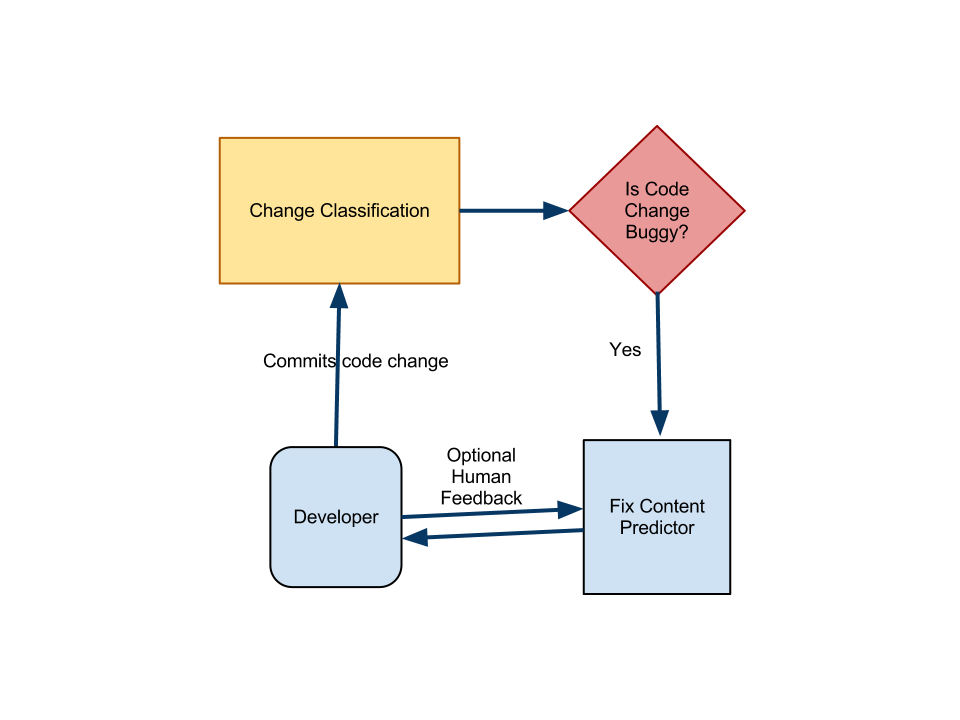
\includegraphics[scale=0.3]{pictures/FixPredictionWorkflow.png}
\end{center}
\caption{Fix Content Prediction Workflow}
\label{workflow}
\end{figure}

\jim{* In figure 1, replace the "developer" box with a stylized graphic of a human}
\jim{Section III.B needs to have, very close to the beginning, a description of the overall approach (that is, the algorithm in Algorithm 1 and the diagram in Figure 2.) At present, this section has references to different steps in the Fix Prediction approach, but these are given without first giving a cross-reference to Algorithm 1, and without giving a high-level description of this algorithm. Once you have given this overview, then the rest of the section can be structured as a walkthrough of the various steps.}

\jim{* Figure 1 looks bad. Bottom of figure is chopped off. The developer feedback lines need to be straight, not slanted. "Commits code change" needs to be two lines, and to the right of the line. There should be a "no" arc on the "Is Code Change Buggy" The outlines on boxes need to be thicker, so they don't look uneven.}

We describe our approach to predicting contents of a bug fix, augmented by change classification, and powered by human feedback.
Contents of a bug fix consist of unordered programming language tokens in a bug fix.
In this paper, contents of a bug fix are synonymous with the terms of a bug fix. These are in turn synonymous with bug fix suggestions. \jim{This needs to be handled more carefully. The typical reader will think of a bug fix as a series of *ordered* programming language statements that change a given source code file. What you are doing is *explicitly redefining* this. The typical setup for this situation is to reaffirm the standard definition, then note how you're going about redefining it.}

An overview of the workflow \jim{*which* workflow? Need some adjectives in there.} is depicted in figure~\ref{workflow}. The steps of the process are:
\begin{enumerate}
\item A code change is submitted.
\item A prediction is made on whether the entire change is buggy or clean using change
classification~\cite{Kim2007p58, shivaji2009reducing}. Change classification is explained in Section~\ref{ChangeClassification}.
\item If the code change is predicted to be buggy, predict contents of a future bug fix to this change.
The predicted fix terms are presented to the user. Fix content prediction algorithm is described in
Section~\ref{FixPred}.
\item The user optionally can provide feedback on the change classification process, improving the prediction models for future changes. The human
interaction process is described in section \ref{HumanFeedbackProcess}.
\end{enumerate}

The next subsections describe proposed steps in detail. 

\subsection{Change Classification}
\label{ChangeClassification}
Change classification is an algorithm used to label and predict code changes as buggy or clean~\cite{Kim2007p58, shivaji2009reducing}. 
The aim of the change classification is indicating
whether a particular code change is buggy or clean.
The key steps of the algorithm are briefly described in this section.
For a detailed
description of the algorithm, refer to~\cite{Kim2007p58, shivaji2009reducing}. \jim{* Section III.A - first two sentences of this section say the same thing. The two cites to [19, 28] in the section should be reduced to just one occurrence.
}
\jim{* When citing a sub-subsection, I recommend III.A(1) - i.e., put the sub-subection heading in parens.}


The primary steps involved in performing change classification 
%on a single project 
are outlined as follows: 
\begin{enumerate}
\item File level changes are extracted from the revision history of a project,
as stored in its SCM repository. 
\item The bug fix changes for each file are identified by examining keywords
in SCM change log messages or cross-referencing with a bug tracking
database such as Bugzilla. 
\item Bug-introducing and clean changes at the file delta level are identified
by tracing backward in revision history from bug fix changes~\cite{Sliwerski2005} as described in Section~\ref{FindingBuggyCleanChanges}.
\item Features are extracted from all changes, both buggy and clean. Features
can include all terms in the complete source code, the lines modified
in each change (delta), AST metrics, and change
metadata such as author and change time as listed in Section~\ref{FeatureExtraction}
\item Historical code change data with features and labels (buggy or clean) can be used to train a classifier. The classifier can then
predict if future changes are buggy or clean.
\end{enumerate}

\subsubsection{Finding Buggy and Clean Changes}
\label{FindingBuggyCleanChanges} In order to find bug-introducing
changes, bug fixes must first be identified by mining change log messages.
We use two approaches: searching for keywords in log messages such
as ``Fixed\textquotedbl{}, ``Buggy\textquotedbl{} {[}4{]}, or other
keywords likely to appear in a bug fix and searching for references
to bug reports like ``\#42233\textquotedbl{}. This allows us to identify
whether an entire code change transaction contains a bug fix. If it
does, we then need to identify the specific file change that introduced
the bug. The bug-introducing change identification algorithm proposed
by Sliwerski, Zimmermann, and Zeller (SZZ algorithm)~\cite{Sliwerski2005}
is used in the current paper. After identifying bug fixes, SZZ uses
a difference tool to
determine what changed in the bug fixes. SZZ tracks down the origins of the modified hunks in the bug fix. The discovered origins are labeled as buggy changes.

\jim{* There are a few missing section cross-references in the paper - search for "??"}


\subsubsection{Feature Extraction}
\label{FeatureExtraction} A commit to a source code repository involves
two source code revisions (an old revision and a new revision) and
a change delta that records the added code (added delta) and deleted
code (deleted delta) between the two revisions. A commit has associated
meta-data, including the change log, author, and commit date. Every
term in the source code, change delta, and change log texts is used
as a feature. Eight features are gathered from commit meta-data: author,
commit hour, commit day, cumulative change count, cumulative bug count,
length of change log, changed LOC (added delta LOC and deleted delta
LOC), and new revision source code LOC.

To generate features from source code, we use a modified version of
the bag-of-words approach (BOW), called BOW+, that extracts operators
in addition to all terms extracted by BOW~\cite{Kim2007p58}, since
we believe operators such as !=, ++, and \&\& are important terms
in source code. We perform BOW+ extraction on added delta, deleted
delta, and new revision source code.

For this paper, select AST features were added to the typical change
classification algorithm. The change distilling algorithm proposed by
Fluri et al.~\cite{Fluri2007} was used to extract the difference between abstract
syntax trees (ASTs) built from the old and new revisions for each commit. The change distilling algorithm categorizes changes
of ASTs into 48 types, according to the taxonomy defined by their
previous work~\cite{Fluri2006}. The number of occurrences
for each change type was used as a feature.

Once the features are extracted and training is performed on sufficient revisions, a new code change can be classified as buggy or clean. The next section introduces
an approach to predict bug fix content for a predicted buggy change.

%\sung{It seems like this is our new contribution. Why it is in the background?}

\subsection{Fix Content Prediction}
\label{FixPred} 

\jim{I like the overview of fix content prediction found at the start of section III.B, and wonder whether this might be moved earlier in the paper, perhaps even into the introduction, or into the section where true and false positives are defined.}

The goal of fix content prediction is to accurately predict code tokens of a future bug
fix to a presented buggy code change.
We denote a buggy revision as B\textsubscript{n}. The corresponding fix to this revision F\textsubscript{n} occurs later in time.


%Fix content prediction aims to predict tokens of F\textsubscript{n} given revision B\textsubscript{n} and all prior revisions.

The inputs to fix prediction are:
\begin{itemize}
\item A code change predicted to be buggy, revision B\textsubscript{n}.
\item All previous revisions annotated with the help of the SZZ algorithm, powered by changelog messages or bug tracking systems as buggy, a bug fix, or neither.

% 
% A map of prior buggy to fix revisions from project history. For example,
% bug inducing revision B\textsubscript{1}and fix revision F\textsubscript{1}(which
% fixes revision B\textsubscript{1}) are given as a map element. 
% \sung{We may need to introduce this earlier. Perhaps, add a diagram to explain it clearly.}
% A
% buggy revision can have one or more fix revisions. For each
% revision, the full set of features are present. 
% \item Code changes which are neither a bug or a fix.
\end{itemize}

The output is a set of code tokens that are likely to be present in revision
F\textsubscript{n}. A good fix prediction will have a high intersection among
predicted tokens and the actual tokens of F\textsubscript{n}. In addition, a good
prediction will have a low false positive and false negative rate.
The former means that there are not too many predicted fix tokens which are not
present in F\textsubscript{n}. The latter means a high percentage of code
tokens in F\textsubscript{n} were amongst the predicted fix tokens.

A function that links tokens of B\textsubscript{n} to the tokens of F\textsubscript{n} is desirable for predicting fix content accurately.
As most of the features extracted are keyword features, a link between buggy and fix keywords is helpful. This work focuses on
statistical approaches to link buggy and fix tokens.

When limited to statistical approaches, one has to exploit
patterns amongst buggy and fix keywords, meta-data, and AST features.
Each of these features can have largely differing sets of values. With differing
value ranges, it is challenging to construct a relationship between
features of a bug and a bug fix. 

The next section
deals with pre-processing features so that their value ranges are
comparable.

\subsubsection{Feature Pre-processing}
\jim{* Section "Feature preprocessing" - I'm not sure what is meant by, "Keyword features can potentially
have a large range of values,"  Is this the range of the keyword counts can be large? Or is this the total number of distinct keywords is large? Need to be explicit.}

\jim{I think it might be cleaner to move the section on Feature Pre-processing (III.B.1) to just after III.A.2 (i.e., just after the feature extraction section). This way we'd talk about feature extraction, and then right afterwards, feature pre-processing (keeping feature manipulation things together). Be sure to change the final sentence in the section.}

Keyword features
can potentially have a large range of values, as
a count of the number of times of occurrence of a particular keyword
in a code change can be used as input from the feature extraction process.
There is a choice on how to interpret this feature, one can either
record the presence of a keyword feature or record the number
of times the feature appears in a code change. 

For example, if a variable maxParameters is present anywhere in the
project, a binary interpretation of this feature records this
variable as being present or absent, respectively 1 or 0 for a code change. A count interpretation would instead
record the number of times it appears for a particular code change. It
was observed that large values when using count tended to skew bug fix
prediction. Employing a binary interpretation additionally allows
one to simplify fix prediction to the presence of a keyword in a code change, instead of the number of times a keyword will appear in a fix.
Thus, a binary interpretation was used for keyword features. This limits
the range of values to 0 and 1 for keyword features.

Numeric meta-data features such as LOC, cumulative change count, cumulative
bug count, length of a change log can have unpredictable ranges as
well. These were numerically scaled to the [0, 1] range using rudimentary scaling transformations~\cite{saunders1998support}. 

AST features presented a different challenge. While AST feature values
do have a large range of values, the range is much smaller than keyword
features. These were scaled to the [0,1] range, similar to numeric meta-data
features.
\jim{Paragraph "AST features presented a different challenge" ... and then start of next paragraph "Categorical features.... represent a different challenge." Too repetitive, change one.}
Categorical features such as author name, commit hour (0-23), and
commit day (1-7) represent a different challenge. One cannot conclude
that a code change committed at 2pm is twice as important as a 1pm
code change. These features were converted to binary terms. For example
if commit day is 2, commit\_day\_is\_2 would be 1 and commit\_day\_is\_1,
commit\_day\_is\_3, .., commit\_day\_is\_7 will all have zero values.
The benefit of using binary values for these features is removing
any numerical bias during analysis. 

The data is now transformed to the [0,1] range. The next section
details the bug fix matrix, an approach that predicts bug fix content using the modified data.

%\subsubsection{Performance Metrics}
%\sung{Put this on in the set up?}
%\label{PerformanceMetrics}

%\subsubsection{Classifier Based Fix Content Prediction}
%\label{Classifier_Fix_Prediction}
%\sung{This is already mentioned, right? we only predict buggy content in the buggy change, right?}
%
%Let's say we start with the first 50\% of project history and want
%to predict fix content in the next 50\% of project history. How exactly
%would one do this? One can start with the important reasons for a
%bug. In other words, the features most responsible for the code change
%being a bug. 
%
%The SVM classifier was used to generate reasons for bugs.
%It was trained on a ratio of project history and tested against the
%rest of history. A linear SVM classifier was used to get feature weights.
%Specifically, Liblinear \cite{fan2008liblinear} was used to obtain the primal weight
%vector w. w can be used as input to predict bug fix content. The algorithm
%used to predict bug fix content is outlined in algorithm \ref{Algo1}.
%\sung{So we are using internal information of SVM to prediction features/contents?}
%
%\sung{Before showing the algorithm, I would sketch the idea first.}
%\begin{algorithm}
%
%\begin{enumerate}
%\item A set amount of revisions from project history, e.g. p\% is used as
%the train set.
%\item The rest of project history is used as the test set, e.g. (100 - p)\%.
%\item Train a classifier on the train portion of history, from step 1.
%\item Get feature weights from the w vector of an SVM.
%\item Sort the features in decreasing order.
%\item Insert the top n\% of features from this list into imp\_set.
%\item For a buggy revision, B\textsubscript{1} in the test\_set, if it
%contains changes from the imp\_set, predict that the same element
%will show up in bug fix, F\textsubscript{1} which fixes revision
%B\textsubscript{1}.
%\end{enumerate}
%\caption{Classifier Based Fix Content Prediction}
%\label{Algo1}
%\end{algorithm}

%The algorithm starts with a set of bug inducing and clean revisions from p\% of project history as the train set. A linear SVM classifier is run on the train set. A linear classifier is used for prediction speed and simplicity. The primal vector weight vector w is returned from the output of Liblinear. The features returned by the weight vector are then sorted in decreasing order. How many of the top features to retain for the imp\_set is a good question for empirical analysis. In the experiments that follow, n was set to be 25\%. Experimentation with higher and lower numbers indicated that this can actually be a tradeoff for precision and recall of fix prediction. More details on this will follow in section YYYY. Finally, if a buggy revision in the test set has a keyword present in the imp\_set, the fix predicted for this change will also contain the same keyword. 
%
%This technique uses a classifier \sung{SVM? Can we use other classifiers for this?} to identify the important features of buggy and fix inducing code changes. It then ascertains that an important feature found in the buggy code change will also be present in its fix. A few questions arise:
%
%\begin{itemize}
%\item How can one predict fix keywords which were never present in the bug inducing change?
%\item How much importance should one place on a buggy change when compared to a bug fixing change?
%\end{itemize}
%
%\sung{This seems a bit off topic at this point.}
%Predicting fix keywords that were not present in the original bug is useful. Section [sub:Bug-Fix-Matrix] discusses an enhancement to algorithm \ref{Algo1} to predict fix tokens not existing in the original bug inducing change.
%
%The importance of a buggy change and a fix may not necessarily be the same. Both buggy and fix changes are only a small percentage of overall changes. The majority of the changes are neutral as can be seen from table \ref{tab:projects}. In the data sets, 27.9\% of code changes on average were bug inducing, 17.5\% were fixes, with the remaining 54.6\% of changes being neutral. The aim of the classifier in algorithm 1 is to predict fix context for a buggy change. If the neutral changes are discounted, there is still a 1.5 to 1 ratio among buggy changes and fix changes. That means the classifier by default would value a buggy change 1.5 times as much as a fix change. This can negatively affect fix content prediction. In order to not bias the classifier towards buggy changes or fix changes, the weights were set so that the overall importance of buggy changes and fix changes were balanced. In other words, if the ratio of buggy changes to fixes are 1.5 to 1, each fix change is valued 1.5 times as much as a bug inducing change in order to equate the overall comparative value of fix and buggy changes. 
%
%For the support machine classifier, the ratio of class weights is reflected in the cost parameter, C, for the class in question (bug inducing or fix) \cite{fan2008liblinear}. In practice, the right ratio for class weights depends on the cost of a false negative vs a false positive. In the case of fix prediction, its the cost of missing a bug fix suggestion compared to the cost of returning errant bug fix terms. A balanced cost keeps the analysis simple at this stage. A future refinement to this work can be experimenting with different weights to improve fix prediction.
%
%The next section introduces the bug fix matrix, which addresses the problem of predicting fix tokens not present in the buggy change.

\subsubsection{Bug Fix Matrix}
%TODO: Remove classifier based bug prediction section and mention it in this.
%The limitation of the classifier based approach of section \ref{Classifier_Fix_Prediction} is the lack of a relationship between buggy and fix relations allowing it to predict fix content not present in the buggy change. 

The Bug Fix matrix generates a link among past buggy and fix revisions. \jim{* Section, "Bug Fix Matrix" -- this section starts with, "The Bug Fix matrix generates a link
among past buggy and fix revisions." That's too vague. What is really going on is you are developing a set of conditional probabilities between buggy keywords and fix keywords.
} It can then be used to predict tokens of a new buggy revision.
\jim{* I think it makes sense to give an example of the Bug Fix matrix first in this section, then go into the details on how it was computed.}
\jim{So:
* overall rationale for bug fix matrix and overall high level description
* example of bug fix matrix
* description of how it was computed}

Section~\ref{FeatureExtraction} generates a vocabulary of features from the first 500 revisions for each project in the corpus.
This vocabulary of features is used by buggy, fix, and neutral revisions. The Fix matrix generates a buggy to fix frequency map between all terms of the vocabulary.
Feature i represents a particular feature of the vocabulary. The left column of the matrix represents the token from a buggy code change.
Each row of the matrix indicates the number of times a token shows up on the bug fix given presence of a token in the buggy change. For example,
 ${M_{i,j}}$ = 1 means that for all buggy changes where token i was present, in only one of them token j was present in the bug fix. The Fix matrix
  can mention how often the same token i occurred in both the buggy change and the fix via ${M_{i,i}}$.

Suppose we had the following three keywords in
a few code changes: File, File.open(), File.close(). A possible fix
matrix is depicted in Figure~\ref{fig:example}. \jim{"A possible fix matrix is depicted in Figure II" -- this is actually Table II.}

\begin{table}\centering
\begin{tabular}{|c|c|c|c|}
\hline 
 & File & File.open() & File.close()\tabularnewline
\hline
\hline 
File & 2 & 0 & 1\tabularnewline
\hline 
File.open() & 0 & 0 & 1\tabularnewline
\hline 
File.close() & 1 & 0 & 0\tabularnewline
\hline 
\end{tabular}

\caption{Bug Fix Matrix Example}
\label{fig:example}
\end{table}

The matrix means that if there is a \textquotedbl{}File\textquotedbl{}
keyword in the bug, amongst all the bug fixes, ``File.close()''
was present once in the bug fix. The bug fix in 2 cases added/modified
``File'' and in one case added a ``File.close'' when ``File''
is in the bug inducing change. When ``File.open()'' was present
in the bug, the bug fix added a ``File.close()''. The matrix reflects
a bug when a developer opens a file but forgets to close it. The bug
fix calls File.close().

\begin{figure}[t]
\begin{center}
 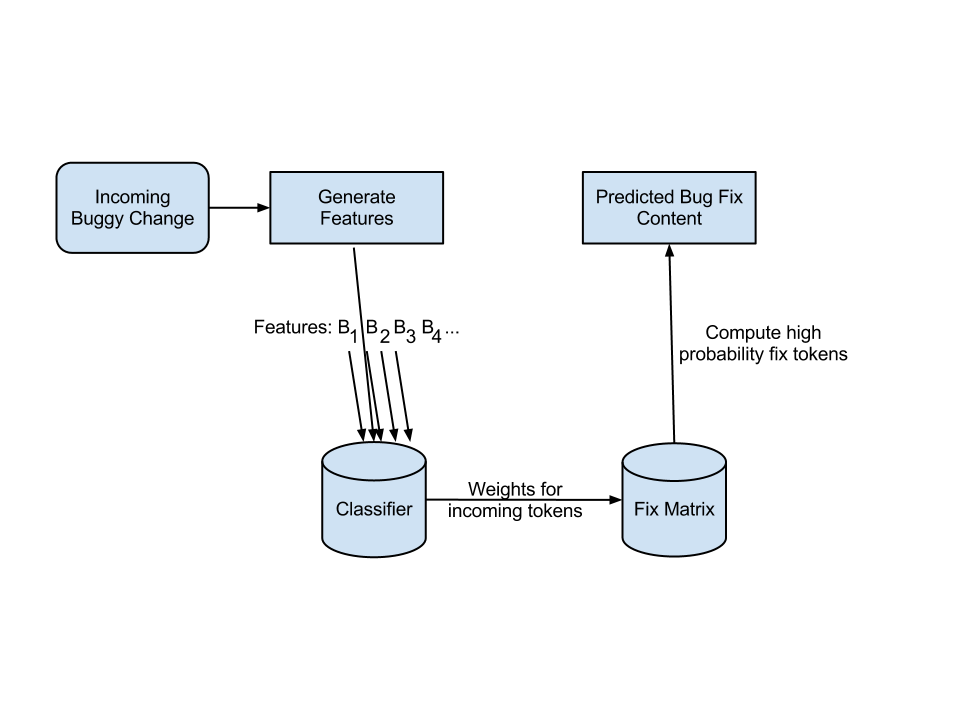
\includegraphics[scale=0.3]{pictures/FixPredictor.png}
\end{center}
\caption{Fix Predictor}
\label{FixPredictor}
\end{figure}

The bug fix matrix can be used to predict
fix content for an incoming buggy change.
\begin{algorithm}
\begin{enumerate}
\item Create a fix matrix on the training set of bug inducing changes and
their respective fixes.
\item Scale every row of the fix matrix to the [0,1] range.
\item Calculate the probability of occurrence in the bug fix for every token in the vocabulary.
\item For a new bug inducing code change, use the bug prediction classifier to produce weights for incoming buggy features.
\item Multiply the probability of each predicted fix token by the classifier weight for the source buggy feature if it exists.
\item Store all candidate fix tokens in imp\_set.
\item Sort the list of features in imp\_set by their probability.
\item Return high probability fix tokens from imp\_set.
\end{enumerate}
\caption{Fix Content Prediction Algorithm}
\end{algorithm}


The fix matrix entries are scaled in step 2 to avoid bias against frequently occurring tokens. Restricting all tokens to the [0,1] range simplifies future predictions.

The classifier is used in step 4 to refine the fix matrix. 
While the fix matrix treats all bug tokens with equal important when predicting fix tokens,
the bug prediction classifier can calculate the importance of a buggy token. As the classifier differentiates buggy changes from clean ones,
the classifier also knows which tokens are most important when distinguishing code changes. The classifier's buggy token weights
were used to boost the probability that fix tokens addressing more important buggy tokens were returned. In other words,
the classifier helps filter out less important buggy tokens, improving the quality of predicted fix tokens.
Details on how the classifier was used to filter out less important buggy tokens follow. Diagram \ref{FixPredictor} outlines the process.
\jim{The paragraph starting: The classifier is used in step 4 to refine the fix matrix. If I understand this paragraph, and the following one correctly, all you are doing is taking the weight for a particular token in the SVM and multiplying that times the raw fix matrix values for that keyword. If so, I don't see why it takes two paragraphs to say that. Instead just write: In step 4, the fix matrix entries are adjusted using information from the classifier used in change classification. The SVM algorithm assigns a weight to each feature, with a higher weight indicating that this feature is more useful in separating buggy changes from clean changes. We assume that these same features are also more useful for predicting which keywords will appear in bug fixes as well, and hence we wish to emphasize these keywords in the fix matrix. To accomplish this, we multiply each matrix entry associated with a keyword by its SVM weight (as found in the SVM primal weight vector w in the Liblinear implementation [12]).   One question I have is this -- for each token you have an entire row of values in the fix matrix. How do you assign a value to each individual token from the row of values. Do you just sum all of the row entries to compute the value for a given token?}

A linear SVM classifier, specifically Liblinear \cite{fan2008liblinear}, was used for bug prediction.
Feature weights were extracted by using the primal weight vector w. w was used as input to the bug fix matrix for an incoming buggy change.
Every feature present present in an incoming buggy change is hereby referred to as an incoming buggy feature. The probability of
every fix token emanating from an incoming buggy feature is multiplied by the buggy feature weight.
The more positive the weight of an incoming buggy feature, the likelihood increases that the predicted fix tokens will address that buggy feature.
An analogy is a human expert who focuses on fixing the critical sections of a buggy code change. The classifier is in essence returning statistically critical buggy tokens.

Once the probability of being a fix token is computed for all tokens in the vocabulary, the bug fix matrix requires a good cutoff for the final step.
A conservative cutoff of the 75th percentile value for the high probability fix tokens was chosen. The results of using the fix matrix are summarized in section \ref{FixContentPredictionResults}.
%If no token predictions in the fix matrix for a given bug inducing token scored above the cutoff.
%The fix matrix itself is an optional step which improves the coverage of fix content. In experiments, the fix matrix was typically found to improve recall at a small cost to precision.
%The results of using classifier based bug prediction along with the fix matrix are summarized in section YYYY.

A practical issue encountered before predicting a bug fix for a buggy code change is one may not know a particular code change is buggy to start with.
The SZZ algorithm for example, traces backward from a bug fix to a buggy change.
Not knowing if a change is buggy until a bug fix is performed would mean that fix content prediction itself could be less useful in practice.

However, the benefit of using a classifier driven approach is one can leverage previous work to make a buggy/clean prediction on a code change and return fix content
 only on those code changes which the classifier thinks are buggy.
The code change classifier performed well on all corpus projects, when training on a ratio of project history to predict if future code changes are buggy or clean. \jim{"when training on a ratio of project history" -- I'm not sure what you mean by "ratio of a project history"}
A separate classifier was used for each project.
It is possible to use an entirely different bug prediction algorithm to predict if a code change is buggy before applying fix prediction.

While the results of fix content prediction in section \ref{FixContentPredictionResults} are a good start in the tough area of fix content prediction, one has not yet engaged a key resource,
the users of the system. \jim{Paragraph starting, "While the results of fix content selection..." through the end of the section. These paragraphs are really about the human feedback process, and hence should be placed in that section (III.C)}
Predictions are ultimately going to be acted on or discarded by humans.
Too many discarded predictions will discourage humans from using the system in the future.
It is important to both engage humans and enable them to improve fix prediction.
%Enabling humans to better understand their software project would be an important bonus.

In many other fields, combining the power of man and machine has yielded much fruit.
Many internet firms use human feedback in various capacities to improve their product, e.g. Google, Yahoo, Microsoft, Ebay, and Amazon.
In the game of chess, even an average chess player combined with a strong machine can dominate machine alone.
This has lead to increased popularity in advanced chess tournaments where centaurs, man and machine combined, compete against each other for prizes \cite{kasparov2010chess}.
Gary Kasparov, a former world chess champion, has drawn a parallel to the Moravec's paradox by showing that human and computer skills complement each other in chess.
He stated that in positions where computers are good, the humans are weak, and vice versa \cite{kasparov2010chess}.
Moravec's paradox states that simple human intuition is quite hard for machines to emulate \cite{moravec1998will}. However, complex human reasoning is somewhat easier
 for machines to compute. This indicates that humans and machines can aim to complement their skills effectively when solving problems.

Going back to fix prediction, the goal is to use human insights to guide bug fixes and statistical machine power to guide human intuition.
The next section deals with using human feedback to improve fix prediction results.
It is important to note that the next section is optional, one does not need human feedback to perform fix prediction, but is very useful to employ.

\subsection{Human Feedback Process}
\label{HumanFeedbackProcess}

Before attempting human feedback, one has to consider practical constraints. Engineers have hectic day jobs and very little time to spare.
When interacting with engineers from the industry on fix content feedback, it was quite difficult to get time and attention.
Given that human time is expensive, they should only be engaged on the most critical code changes.
Finally, making the feedback intriguing to humans is desirable.
With the limited time available to provide feedback, lack of captivation can rapidly make matters worse.

Algorithm 2 incorporates human feedback for fix content prediction taking into account the above constraints.

\begin{algorithm}
\begin{enumerate}
\item A set amount of revisions from project history, e.g. p\% is used as
the train set.
\item The rest of project history is used as the test set, e.g. (100 - p)\%.
\item Compute the prediction confidence score for each revision of the train set.
The confidence score is how confident the SVM classifier is on correctly predicting a change as bug inducing or clean.
\item Mark the least confident incorrectly classified revision from the train set as a candidate for human feedback.
\item Consult with human on whether the human feedback candidate revision is buggy, a bug fix, neither, or both.
\item Apply algorithm 1 on the new data set.
\item Compare the precision and recall of fix prediction with and without human feedback.
\item Return a score to the human that is function of the delta in both precision and recall.
\item Return to step 3.
\end{enumerate}
\caption{Human Feedback on Fix Content Prediction}
\end{algorithm}

The first two steps are self explanatory. Step three computes the bug prediction confidence score for each revision in the train set.
Bug prediction at this step feels unrelated to fix content prediction.
However, if the probability of a change being buggy is represented as P\textsubscript{Buggy},
and the accuracy of fix content prediction is Pr\textsubscript{Fix},
the overall probability of the fix content being valid is strongly influenced by P\textsubscript{Buggy}.
An extreme case is when P\textsubscript{Buggy} is zero, in which case predicting fix content for that change is meaningless.
While multiplying Pr\textsubscript{Fix} by P\textsubscript{Buggy}
to indicate the overall accuracy of fix content prediction does not necessarily make logical sense, P\textsubscript{Buggy} cannot be ignored.

One of the constraints with human feedback is that humans should be engaged for as short a duration as possible.
While merely change the label of a revision sounds simplistic, it is a low hanging fruit as the results in section \ref{HumanFeedbackResults} show.

\begin{figure}[t]
\begin{center}
 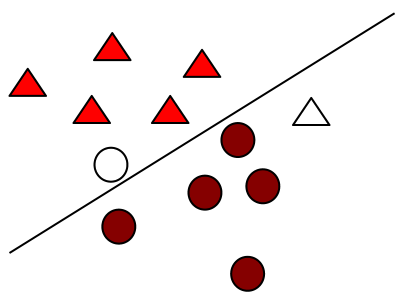
\includegraphics[scale=0.40]{pictures/svm.png}
\end{center}
\caption{Example SVM Classifier in 2D}
\label{example_svm}

\end{figure}

For an SVM based bug prediction classifier, a hyperplane separating bugs from clean changes is built.
Figure \ref{example_svm} depicts a sample hyperplane in two dimensions.
Typically an SVM is more confident of points further away from the hyperplane as opposed to those that are close.
Points that are close to the boundary might easily be misclassified if the current hyperplane needs to be adjusted.
In other words, points close to the hyperplane are most sensitive to a small change in the classifier. In figure \ref{example_svm}, the hyperplane separates triangles from circles. The white circle and triangle are out of place.
 Both of those points are incorrectly classified and are in the wrong side of the separating hyperplane.
 This hyperplane is a line in 2D. If the triangles and circles are buggy and clean revisions, the top candidate for feedback would the revision represented by the white circle.
This revision is picked over the white triangle as it is closer to the separating hyperplane.

Step 3 thus queries the point which the SVM is least confident on, and is incorrect. A question might arise on why are the more confident incorrect revisions not picked at this stage. The reason is to correct revisions one at a time,
while improving classifier confidence gradually, starting from the least confident and proceeding to regions of greater confidence if the human is willing.

Step four proceeds to present this point to humans for feedback.
This is a greedy algorithm as the model is recomputed based on a single point of feedback.
Tong and Koller \cite{tong2002support} show that myopic solutions are commonly used and work well in text classification.
In order to relate this problem to the active learning context,
every buggy/clean label that was derived from SZZ is treated as unlabelled as these points are machine labeled but not commented on by a human.
In step 4, the point most likely to have incorrectly derived label is presented to humans for review.

Non greedy algorithms were also tested in this step and found to perform worse.
An example of a non greedy algorithm is to present the N least confident revisions for human feedback.
Empirically, it was found that presenting five or more least confident revisions to the user for human feedback
was slower than presenting revisions one at a time.

The reason for this can come from an illustrative example. Say there are three revisions, $R_{1}$, $R_{2}$, and $R_{3}$. $R_{1}$ and $R_{2}$ are buggy, and $R_{3}$ is clean. If the classifier is given initial input that all revisions are clean,
 and it's confident that not all revisions should be clean, it can ask for human feedback. A human can give feedback one revision at a time or multiple revisions at a time. If the classifier deems that it is least confident on $R_{1}$,
  it can request feedback on it. Once a human labels that revision as buggy, the classifier might be able to deduce that revision 2 is buggy as well, and complete the cycle of feedback. In contrast,
  if the classifier returns the top two revisions that its less confident about, i.e. revision 1 and 2, a human would have to waste time evaluating revision 2. Being greedy gathers and applies feedback one revision at a time.
  It has the benefit that less overall feedback has to be ultimately delivered by a human. Hence the mechanism employed requests feedback for a single revision. \jim{Parargraph starting, "The reason for this can come from an illustrative example." Since you went to the trouble of making R1, R2, R3, these should be used consistently throughout. In some places the document uses R1, R2 and other revision 1 and revision 2.}

\jim{Section V, First sentence -- I think it would be better to call the subjects "subjects" and not "humans" which sounds a bit impersonal (global change in this section). Also, the wording is a bit off:}

Humans have a choice to label this revision as buggy, a bug fix, both, or neither.
Several code changes are both a buggy and a fix when using SZZ.
Human participants were allowed to look at the fix of the bug and the code change that it fixed in the case of a bug fix.
Human participants were only allowed to look a revisions in the train set. It is important to keep the test set totally hidden to not bias results.
The correct judgment of a code change was left entirely up to human discretion.

A score is returned back to the human after every feedback.
This serves a dual purpose, to track the delta over a purely machine driven fix prediction algorithm
and to provide more motivation for humans to deliver feedback.
The computed score is the sum of the precision and recall improved over the machine only fix prediction approach.
The exact formula is $$score = M* (Pr_{FPH} - Pr_{FPM} + R_{FPH} - R_{FPM}) $$ where $Pr_{FPH}$
is the precision of fix prediction when given human feedback and $Pr_{FPM}$
is the precision of fix prediction for the machine driven approach.
Correspondingly, $R_{FPH}$ and $R_{FPM}$ are the recall of the fix prediction process when driven by humans and machines respectively.
M is a multiplication scaling factor which transforms the score into larger numbers
for better human appreciation. M was set to 10 in the human feedback experiments.

The next section details results from machine based fix prediction and the improvement gained by human feedback.

\section{Results}
\label{Results}
\jim{* Section IV (Results) - there are two section headings in quick succession here, IV.A and IV.B -- either there is a missing section, or there needs to be one less section heading.}


\subsection{Range of Fix Prediction Performance in terms of project history}

\label{RangeFixPredictionPerformanceResult}
\subsection{Results}

\begin{figure}[t]
\begin{center}
 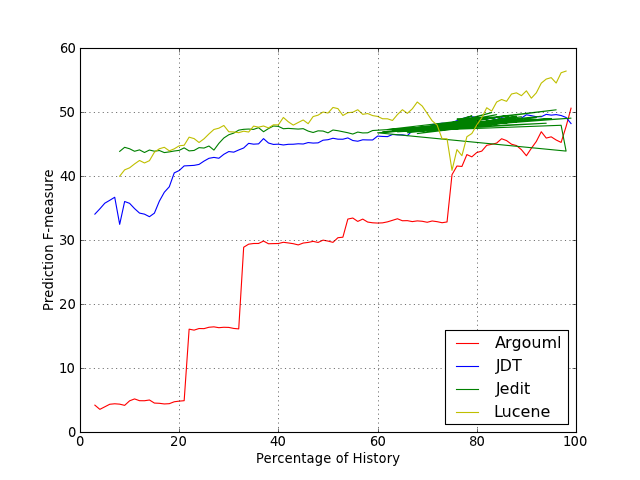
\includegraphics[scale=0.35]{pictures/rq1.png}
\end{center}
\caption{Fix content Prediction F-measure on Project History}
\label{fix_content_machine}

\end{figure}


%\begin{table}\centering
%\caption{Fix Content Prediction rate per project from top 10\% of periods from Project History
%\sung{Why only top 10? How much we can improve by putting humans into to the loop (feedback)?}}
%\label{tab:TopFeedback}
%\begin{tabular}{|c|c|c|c|}
%\hline
%Project &  Precision &  Recall &  F-measure\\
%\hline
%Argouml &  21.97 &  31.07 &  25.67\\
%\hline
%Eclipse &  40.05 &  19.63 &  26.32\\
%\hline
%jEdit &  43.27 &  27.96 &  33.93\\
%\hline
%Lucene &  31.96 &  21.71 &  25.68\\
%\hline
%Average &  34.31 &  25.09 &  27.90\\
%\hline
%\end{tabular}

%\end{table}

\begin{table}\centering
\caption{Average Fix Content Prediction rate per project from Project History}
\label{tab:AvgFeedback}
\begin{tabular}{|c|c|c|c|}
\hline
Project &  Precision &  Recall &  F-measure\\ 
\hline
Argouml &  20.62 &  22.78 &  20.06\\ 
\hline
Eclipse &  32.77 &  17.60 &  21.99\\ 
\hline
jEdit &  29.88 &  22.40 &  24.79\\ 
\hline
Lucene &  25.59 &  19.25 &  20.82\\ 
\hline
Average &  27.22 &  20.51 &  21.91\\ 
\hline
\end{tabular}

\end{table}

Machine based fix prediction was evaluated by training on p\% of project history and testing on (100-p)\% of project histories for p ranging from 1 to 100 in 1 percent increments.
This produces a hundred fix prediction evaluation points per project.
Machine based fix prediction is able to achieve an average precision of 27.2\% and
a recall of 20.5\% when averaging the evaluation points over all projects in the corpus. Table \ref{tab:AvgFeedback} contains averaged results by project. Figure \ref{RangeFixPredictionPerformanceResult}
 depicts a historical graph of predicted fix content F-measure vs ratio of project history. Unsurprisingly, the best fix content prediction
 occurs during the middle periods in history. It is encouraging that after 1-2\% of project history, fix prediction F-measure rises significantly.
Overall, predicting bug fix content is a hard problem. Being able to correctly predict 27\% of the actual content of bug fixes while covering 20\% of all bug fix tokens is not a bad start.


\subsection{Effect of Human Feedback on Fix Prediction}
\label{HumanFeedbackResults}

\begin{table}
\caption{Average Human Feedback Results after 10 revisions per project}
\label{tab:humanFeedback}
\begin{tabular}{|c|c|p{2.3cm}|}
\hline 
Project & Precision Gain & \% Recall Gain\\
\hline 
Argouml & 40.75 & 23.55\\
\hline  
Eclipse JDT & 3.02 & 6.59\\ 
\hline 
Jedit & 4.65 & 4.70\\
\hline  
Lucene & 4.19 & 0.43\\ 
\hline 
Average & 13.15 & 8.82\\
\hline 
\end{tabular}

\end{table}

%While machine generated feedback gives an average of 27.2\% precision and 20.5\% recall in all projects.
%Machine generated feedback on the top 10\% points of project history returned an average precision of 34.3\% and an average recall of 25.1\%. Will update results with graph.

Human feedback gave an average improvement of 13.2\% precision and 8.8\% recall over machine generated fix prediction results after feedback was given on only 10 revisions!
This is a surprising result indicating that even minute feedback can be very beneficial. Table \ref{tab:humanFeedback} depicts the improvement by project.
Humans were restricted to providing feedback on the first half of project history, with their feedback being applied on the second half of project history.
Table \ref{tab:humanFeedback} shows a gain in both precision and recall after ten revisions.

Successful human feedback mainly consisted of the following activities.
\begin{description}
\item[Correcting Incorrectly labeled fixes] \hfill \\
These are code changes which are labeled as fixes in the changelog, but are not typical bug fixes.
A few of these fixes included minor fixes to documentation, java docs, and configuration files. There were also bug fixes that were code refactorings.
While these were labeled as fixes in the changelog, human judgment indicated otherwise.
Notably, the machine learner also diagnosed these as likely to be incorrect fixes and suggested during the feedback step that these were incorrectly labeled.

\item[De-emphasizing Minor bug fixes] \hfill \\
A typical minor bug fix observed in a projects is a bug fix that removes compilation warnings.
Humans participating in the study judged the code change as not being a bug fix.
Minor bug fixes were incorrectly lowering the precision and recall of predicting bug fix content.
\end{description}

As human feedback was only used for 10 revisions, lower hanging fruit might have been uncovered. It is possible that as feedback is given on many more revisions, the kind of feedback would be rather different. The
next section details human feedback as a case study.

\section{Human Feedback Case Study}
\jim{Section III.C needs to describe, someplace near the start of the section (after the current first paragraph?) what is going on in the algorithm. Specifically, you are asking engineers to provide feedback on change classification (bug prediction) in order to improve fix prediction. This is an important point, and if it isn't stated up front, people will miss it and be confused.}
\jim{Feedback was conducted on ten *subjects**:* six of are industrial software engineers and four are ...}
\jim{There needs to be more of a description of the study in this paragraph. You need to walk through what happened with each person, like:}

\jim{Each subject was presented with a series of software project revisions. @@@ Do the developers have any prior knowledge of these projects? If not, how are they expert enough to make this judgement? @@@
For each presented revision, the subject was asked to determine the following: if the revision was labeled as a bug fix, the subject needed to verify that it was, indeed a bug fix. If the revision was labeled as a ... (got through the permutations -- what exactly were the set of possible responses the subject could give??) After receiving this feedback, the SVM was re-trained, and a feedback score was computed: positive scores indicate improvement in SVM performance at fix keyword prediction(???) while negative scores indicate a decrease in SVM performance at this task. This feedback score was presented to the subject before continuing on to the next revision.}

Feedback was conducted on ten humans, six of them are engineers working in the industry and four are student researchers or faculty.
Humans were given a score for their feedback during the entirety of their participation. Each participant gave feedback on ten revisions per project, for two different projects.
For some individual human evaluations, there were points of negative score gains in the interim,
before ten revisions were complete. Interestingly, this motivated humans to provide more feedback and improve their score.

Overall, the industrial participants in particular were intrigued during the process of providing feedback which can be used to predict bug fix content.
After the evaluation the participants discussed the possibility of adopting such a system in their daily professional lives. Their concerns are listed below.
\begin{description}
\item[Speed of applying human feedback] \hfill \\
The method provided in the paper can take up to two minutes to apply human feedback and request feedback on the next computed revision.
This is due to the fact that a new SVM is built after human feedback on a particular revision. The bottleneck is computing the next revision for human feedback.
In practice, this can be solved in a variety of ways.
The simplest is to process human feedback asynchronously. The feedback score and the next revision would be sent in an email or by a comparable asynchronous solution.
There is also research on improving active learning speed with support vector machines \cite{glasmachers2008second}.
Finally, using fast non SVM based online learners like Vowpal Wabbit can speed up active learning \cite{langford2009sparse} .
One of the participants indicated that providing feedback on incorrectly labeled fixes especially when the feedback took two minutes to process is boring.
 He mentioned that he would not mind providing feedback on incorrect fixes if the feedback turn around time was a matter of seconds.

\item[Human Feedback score] \hfill \\
When participants see an improved positive score, they get a feeling that their feedback was correct. Conversely, a negative score creates a negative feeling.
In reality, both feelings can be incorrect.
While accurate feedback would converge towards an increased delta on both precision and recall,
it is well possible that during the short-term, negative scores can result from correct feedback.
An example is when there are a few revisions the classifier is not confident on, say R\textsubscript{1}, R\textsubscript{2},
and R\textsubscript{3}. The correct classification is a bug fix for all three, and currently all three are marked as buggy.
If feedback was only provided on R\textsubscript{1}, but not on the others, it is possible that a model with R\textsubscript{1} marked as a bug fix,
but R\textsubscript{2} and R\textsubscript{3} marked as buggy will score worse than the initial machine model of all three marked as buggy.
After feedback is provided on all three revisions, there can be a marked improvement over machine based fix prediction.
An idea worth exploring is displaying revisions that are most responsible for grading human feedback as negative.
\item[Collaborative Feedback] \hfill \\
Incorporating feedback from a few humans on a particular revision can improve the prediction process taking less time away from each human.
Undoubtedly, poor feedback from one or two humans can have an adverse effect on the system.
On the whole, given that human feedback on average substantially improved fix content prediction as shown in table \ref{tab:humanFeedback}, a collaborative feedback model appears promising.
\end{description}

\jim{* Since one of the projects was really above average, and your sample set is small, it might be better to report a mean improvement here, not an average}

\jim{Sentence "Processing human feedback a revision at a time" - this is a sentence fragment.}

\jim{It wasn't clear to me why you felt it was necessary to recompute the SVM after each piece of feedback. Was this to determine how much of an improvement was gathered from that feedback? If so, couldn't you have just gathered the feedback on several changes, and then computed these improvements at the end, once they had finished giving feedback on all 10 changes? As well, it seems that the Human Feedback score wasn't that useful for the participants..}


\section{Related Work}
\label{RelatedWork}

\jim{ I think the related work section should come after the introduction in this paper.}
\par As this paper touches on a few different techniques, related work can be gathered from one of three phases of figure \ref{workflow}. 


\subsection{Bug Prediction on a Given Software Unit} 
\par Several approaches attempt defect prediction on a given software unit. It is ideal for the software unit to be as small as possible. Prediction on a code change allows an individual change to be targeted for fix content prediction. Aversano et al. \cite{aversano2007lbi} use KNN (K nearest neighbors) to locate faulty modules.  Hata et al. \cite{Hata2008} showed that a technique used for spam filtering of emails can be successfully used on software modules to classify software as buggy or clean. Kim et al. \cite{Kim2007p58} and Shivaji et al. \cite{shivaji2009reducing} perform bug prediction on a code change. The latter technique was used by this paper. D'Ambros et al. \cite{d2011evaluating} perform an extensive comparison of various bug prediction algorithms that operate at the file level.

\par While its preferable for the software unit to be as small as possible in order to optimize the future steps in the process, any of the above methods can be used in place of a code change level bug predictor.

\subsection{Bug Fix Content Prediction}

Suggestions for Bug Fixes can come from different techniques. The most common is via static analysis. Related work not using static analysis is also discussed. 

\subsubsection{Static Analysis Techniques}

Predicting bug fix content is a challenging problem especially when
using statistical techniques. The static analysis community has spent
considerable effort in exploiting language semantics to suggest fixes
to bugs. Popular tools using static analysis for fix suggestions
include Findbugs \cite{ayewah2008using}, PMD \cite{rutar2004comparison}, BLAST \cite{muhlberg2007blast}, FxCop \cite{wagner2008evaluation} amongst many others. There are also approaches from literature which do not yet have downloadable tools available. 

Demsky et al. focused on data structure
inconsistency~\cite{demsky_data_2005,demsky_inference_2006}. Their approach
checks data structure consistency using formal specifications and inserts
run-time monitoring code to avoid inconsistent states. This technique
provides workarounds rather than actual patches since it does not modify source
code directly.

Arcuri et al. introduced an automatic patch generation
technique~\cite{arcuri_automation_2008,arcuri_multi-objective_2008,arcuri_novel_2008}. They used genetic programming. Their evaluation was limited to
small programs such as bubble sort and triangle classification.

The method suggested in this paper
approaches the problem statistically. The general benefits of a statistical
driven approach are:

\begin{itemize}
\item A focus on predicting fix suggestions that will actually be fixed in practice. [Ref]
has analyzed static analysis suggestions and found that less than
1\% of the suggestions are actually fixed in practice. When interacting
with a few industrial settings, this number was found to be less than
0.5\%. In contrast, the statistical driven approach presented has a
an average precision greater than 27\%.
\item Project history is leveraged and automatically tailored for adaptive
prediction of bug fixes relevant to the future code changes of a particular
project. Historical trends can also be exploited. If a particular
type of bug fix was popular at the onset of a project but diminished
in significance soon, statistical fix content prediction will downplay
the importance of that fix pattern.
\end{itemize}

There are benefits to static analysis when compared to statistical
approaches including:

\begin{itemize}

\item The suggested bug fix is an exact solution which can often be proved
in its effectiveness. In contrasts, a statistical approach is a probabilistic
statement on the likely contents of a bug fix.

\item The suggested fix and explanations can be well understood by humans.
While human feedback is addressed in this paper to augment a statistical
approach, static analysis based tools such as Findbugs provide human
understandable analysis of fix suggestions by default. Findbugs tries
to help humans understand its analysis. In contrast, the presented
approach aims to improve machine suggestions by understanding humans.

\end{itemize}

\subsubsection{Fix Content Prediction Without Static Analysis}
Nguyen et al. \cite{nguyen2010recurring} recommend bug fixes for a class or method if a fix was applied to a code peer. If a relevant bug fix was applied to a similar class, it is then recommended. Code peers are defined as objects which work in a similar manner when using a graph based representation of object usages.

Summary Memories of Bug Fixes, BugMem ****.

Holmes and Murphy proposed an approach to extract structural components from example code and use them to assist coding when developers are working on similar code \cite{holmes2005using}.

The approach presented in this paper is similar to BugMem and Holmes et al. in that suggestions are made for a particular code change. The difference is that the recommended tokens are continuously validated against actual bug fixes. This ensures that the fix recommendations are likely to appear in actual fixes.

In the field of information retrieval, matrices are often used to represent document similarity \cite{rolleke2006general}. While fix content prediction is a different problem, representing bugs and fixes as problem spaces and relating these spaces using a matrix has a high level parallel. The matrix relating buggy changes to fixes modelled a linear relationship in this paper. Future work can extend the concept to capture more complex relationships between buggy and fix changes.

\subsection{Human feedback}
Human feedback via active learning is well studied by the IR community. Tong et al. utilize human feedback via active learning when using support vector machines for text classification in \cite{tong2002support}. Tang et al. use active learning to improve statistical natural language parsing techniques \cite{tang2002active}. Both studies conclude that using active learning on a small percentage of samples provided as much information as randomly sampling many more data points. 

Active learning was used to classify software behavior in \cite{bowring2004ala}. Bowring et al. \cite{bowring2004ala} mention that classifying software behavior is a process that naturally contains many unlabelled data points with a huge cost to label each of the points. They also indicate that active learning provided results comparable to supervised learning in their experiments.
 
Xiao et al \cite{xiao2005sta} use active learning for modelling software behavior in commercial games. They conclude that actively learning helped achieved good scalability for complex game scenarios while providing useful visual models to humans.

Finally mention Lucia et al. [REF] ****
\jim{Note that there is still a placeholder in related work "Summary Memories of Bug Fixes, BugMem ****." and "Finally mention Lucia et al. [REF] ****"}

Human feedback if performed selectively can provide valuable performance improvements to machine classifications.


\section{Threats to Validity}
\label{ThreatsToValidity}

\par \textbf{Systems examined might not be representative of typical projects.} \\
11 systems are examined, more than any
other work reported in literature. In spite of this, it is still possible that we accidentally chose
systems that have better (or worse) than average fix content prediction accuracy. Since we
intentionally chose systems that had some degree of linkage between change tracking
systems and change log text (to determine fix inducing changes), there is a
project selection bias.

\par \textbf{Systems are open source.} \\ The systems examined in this paper use an open source
development methodology, and hence might not be representative of typical development contexts. It
is possible that more deadline pressure, differing personnel turnover patterns, and varied
development processes used in commercial development could lead to different bug fix
patterns.

\par \textbf{Bug fix data is incomplete.} \\ Even though we selected projects that have decent change logs,
we still are only able to extract a subset of the total number of bugs (typically only 40\%-
60\% of those reported in the bug tracking system). Since the quality of change log comments varies across
projects, it is possible that the output of the classification algorithm will include false positive
and false negatives. It is currently unclear what impact lower quality change logs has on classification results. This affects both feedback and fix predcition.

\par \textbf{Bug introducing data is incomplete.} \\ The SZZ algorithm used to identify bug-introducing
changes has limitations: it cannot find bug introducing changes for bug fixes that only involve deletion of source code.
It also cannot identify bug-introducing changes caused by a change made to a file different from the one being analyzed. It is also possible to miss bug-introducing
changes when a file changes its name, since these are not tracked.

\par \textbf{Selected classifiers might not be optimal.} \\ We explored many
other classifiers, and found that the SVM consistently returned the
best results and has the most suitable infrastructure for fix content prediction and human feedback. It is however possible that another classifier can do a better job.

\par \textbf{Humans consulted for feedback may not be representative.} \\ We selected six people from the industry, and four from academia. It is possible that these individuals provide better or worse feedback
than the typical industrial or academic engineer.


\section{Conclusion}
\par This paper introduces a novel statistical fix content prediction method that can predict unordered tokens of a bug fix. While predicting contents of a fix is a tough problem, the proposed approach is able to predict fix content
on average with 27.2\% precision and 20.5\% recall. Section \ref{fix_content_machine} shows that results can be better than these average figures for many points in a project's history.

\par While these results are promising, it is encouraging that human feedback on as little as ten revisions significantly improves fix content prediction. Table \ref{tab:humanFeedback} shows a 13.1\% precision and 8.82\% recall gain after
humans provided feedback on just 10 revisions per project for 2 projects. The results represent an averaging of human feedback improvement.

\par Predicting the contents of a bug is a tough problem. This paper provides a method that can aid developers with bug fix suggestions that are constantly validated against actual bug fixes. Human feedback plays an important role
not only in improving fix prediction performance but also in helping humans understand machine classification of code changes.

\par In the future, when software developers have advanced bug prediction technology
integrated into their software development environment, the use of a bug fix matrix with a change classifier will permit improved bug fix content prediction. With
widespread use of integrated bug and fix content prediction, future software engineers can
increase overall project quality by catching errors and deploying fixes in reduced time.


% \balance
\bibliographystyle{abbrv}
\bibliography{ase09,faultpred,autofix}

 
\end{document}
